\chapter{Numerical Evaluation: Accuracy and Efficiency}

\label{Chapter7} % Change X to a consecutive number; for referencing this chapter elsewhere, use \ref{ChapterX}

\lhead{Chapter 7. \emph{Numerical Evaluation: Accuracy and Efficiency}}
% We performed experiments on a machine with 4 Intel Xeonr
% Quad-core E7320 processors and 16 GB memory. The operating
% system was Fedora release 9 with kernel 2.6.25. The compiler was
% gcc 4.3.0
Calculations were performed on 12\textsuperscript{th} Gen Intel\textsuperscript{\textregistered} Core\texttrademark{} i5-12500~$\times$~12 core processor
we evaluated the computational efficiency and accuracy of our algorithm and compared it with PHL ewald and also with the method given by kawata et al.
The dimentions of the system were $L_x = L_y = L_z = 25$ \AA . The configuration of the systems were generated randomly using LAMMPS.

\section{Convergence}
We took a system of 10,000 Na and Cl ions in a 25 \AA box for our convergence benchmarking.
Based on our analysis for various gamma values, we calculated the reciprocal space energies for a given system and checked for the convergence of the sum. But due to very high $k_z$ values for the convergence this method becomes more expensive as compared to other older methods because for every iteration of $k_z$ to compute the energy the new structure factor $S(\vec G)$ is computed which increase the time complexity by $O(N)$, so now we will use the particle mesh ewald which doesn't depend on the $k_z$ loop as the bottleneck of that program is grid interpolation which is done outside the energy summation loop.
% \begin{figure}[htbp]
\begin{figure}[H]
    \centering
    \includegraphics[scale=0.4]{images/logerror_vs_kz_forreport.jpg}
    % \includegraphics[width=\linewidth]{images/logerror_vs_kz_forreport.jpg}
    \caption{Convergence of relative errors in $U_{LR}$ with $k_z$ for various values of $\gamma$.}
    \label{fig:result1}
\end{figure}
\section{Particle Mesh Ewald-Modified}
To enhance the efficiency of the calculations, the structure factor was computed using B-spline interpolation employing Fast Fourier Transforms (FFTs). The best accuracy and optimal time of our method+SPME is determined from the combination of gamma, order and grid. smaller the gamma, higher the grid points required for the interpolation. 
\section{Real Space Improvement}
The of the interpolation function gave around 15\% improvement in the calculation time. 
\begin{figure}[H]
    \centering
    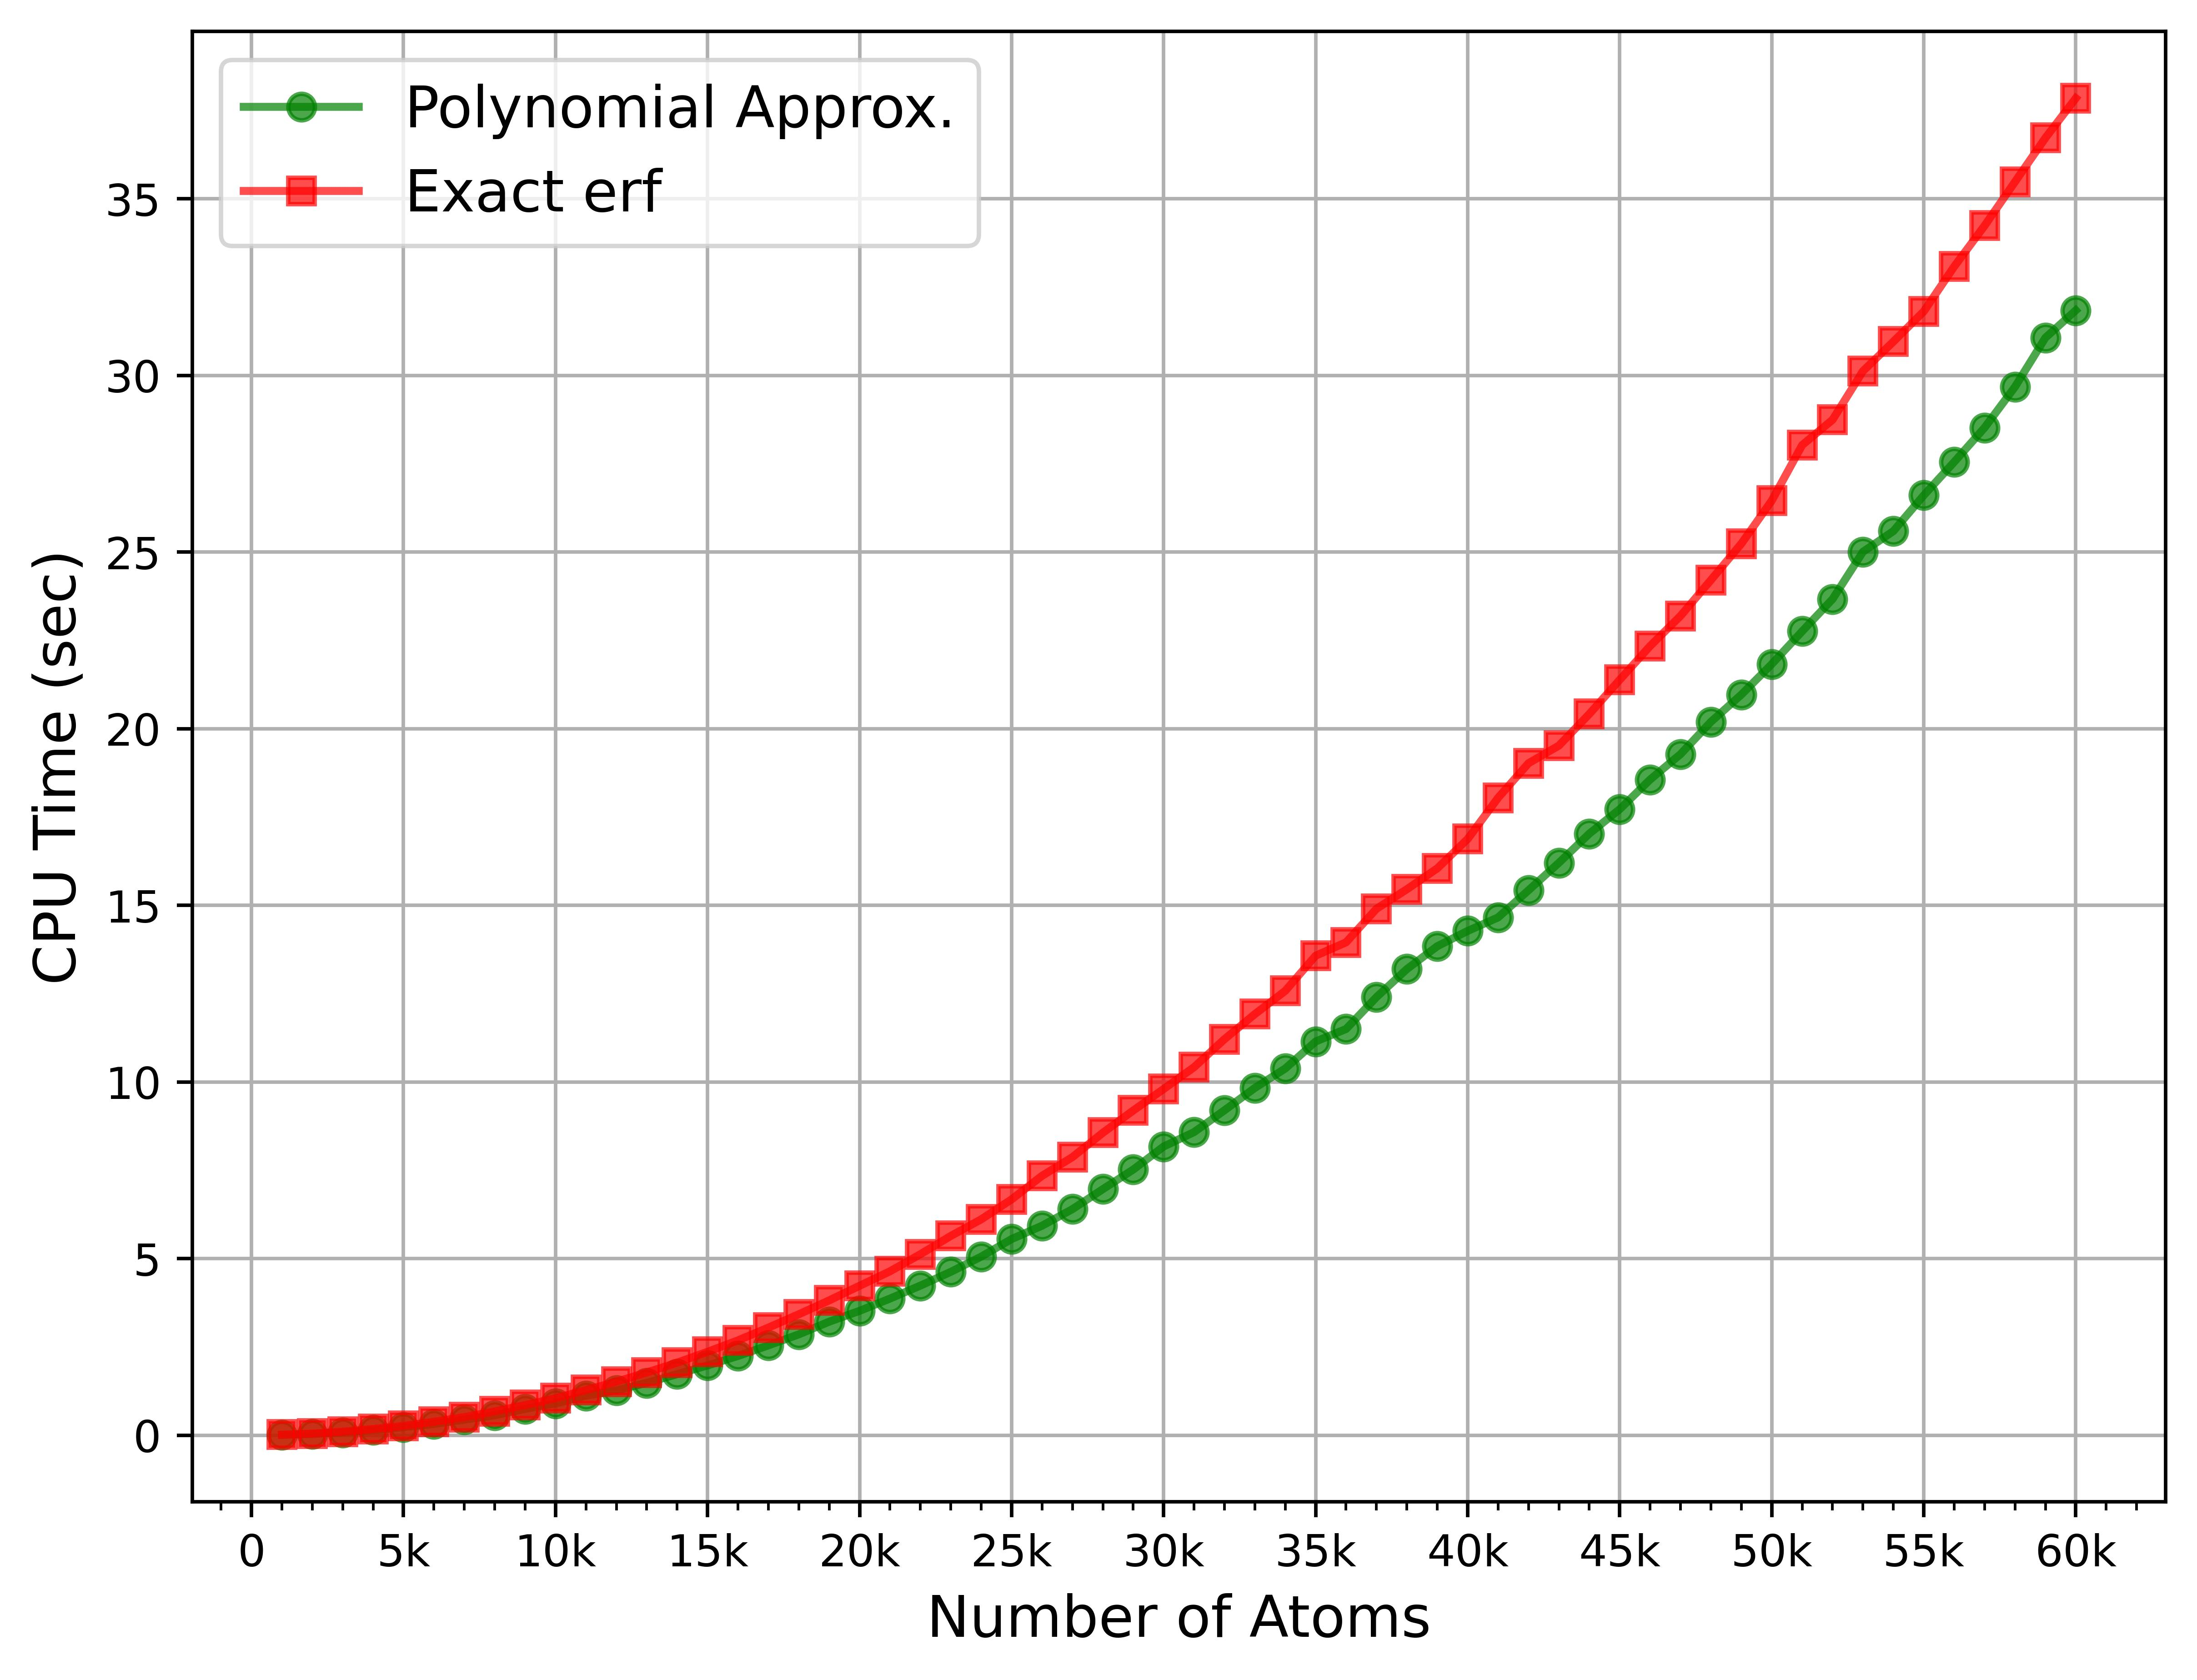
\includegraphics[width=0.75\linewidth]{images/realspaceopt.jpg}
    \caption{Enter Caption}
    \label{fig:enter-label}
\end{figure}
\begin{figure}[H]
    \centering
    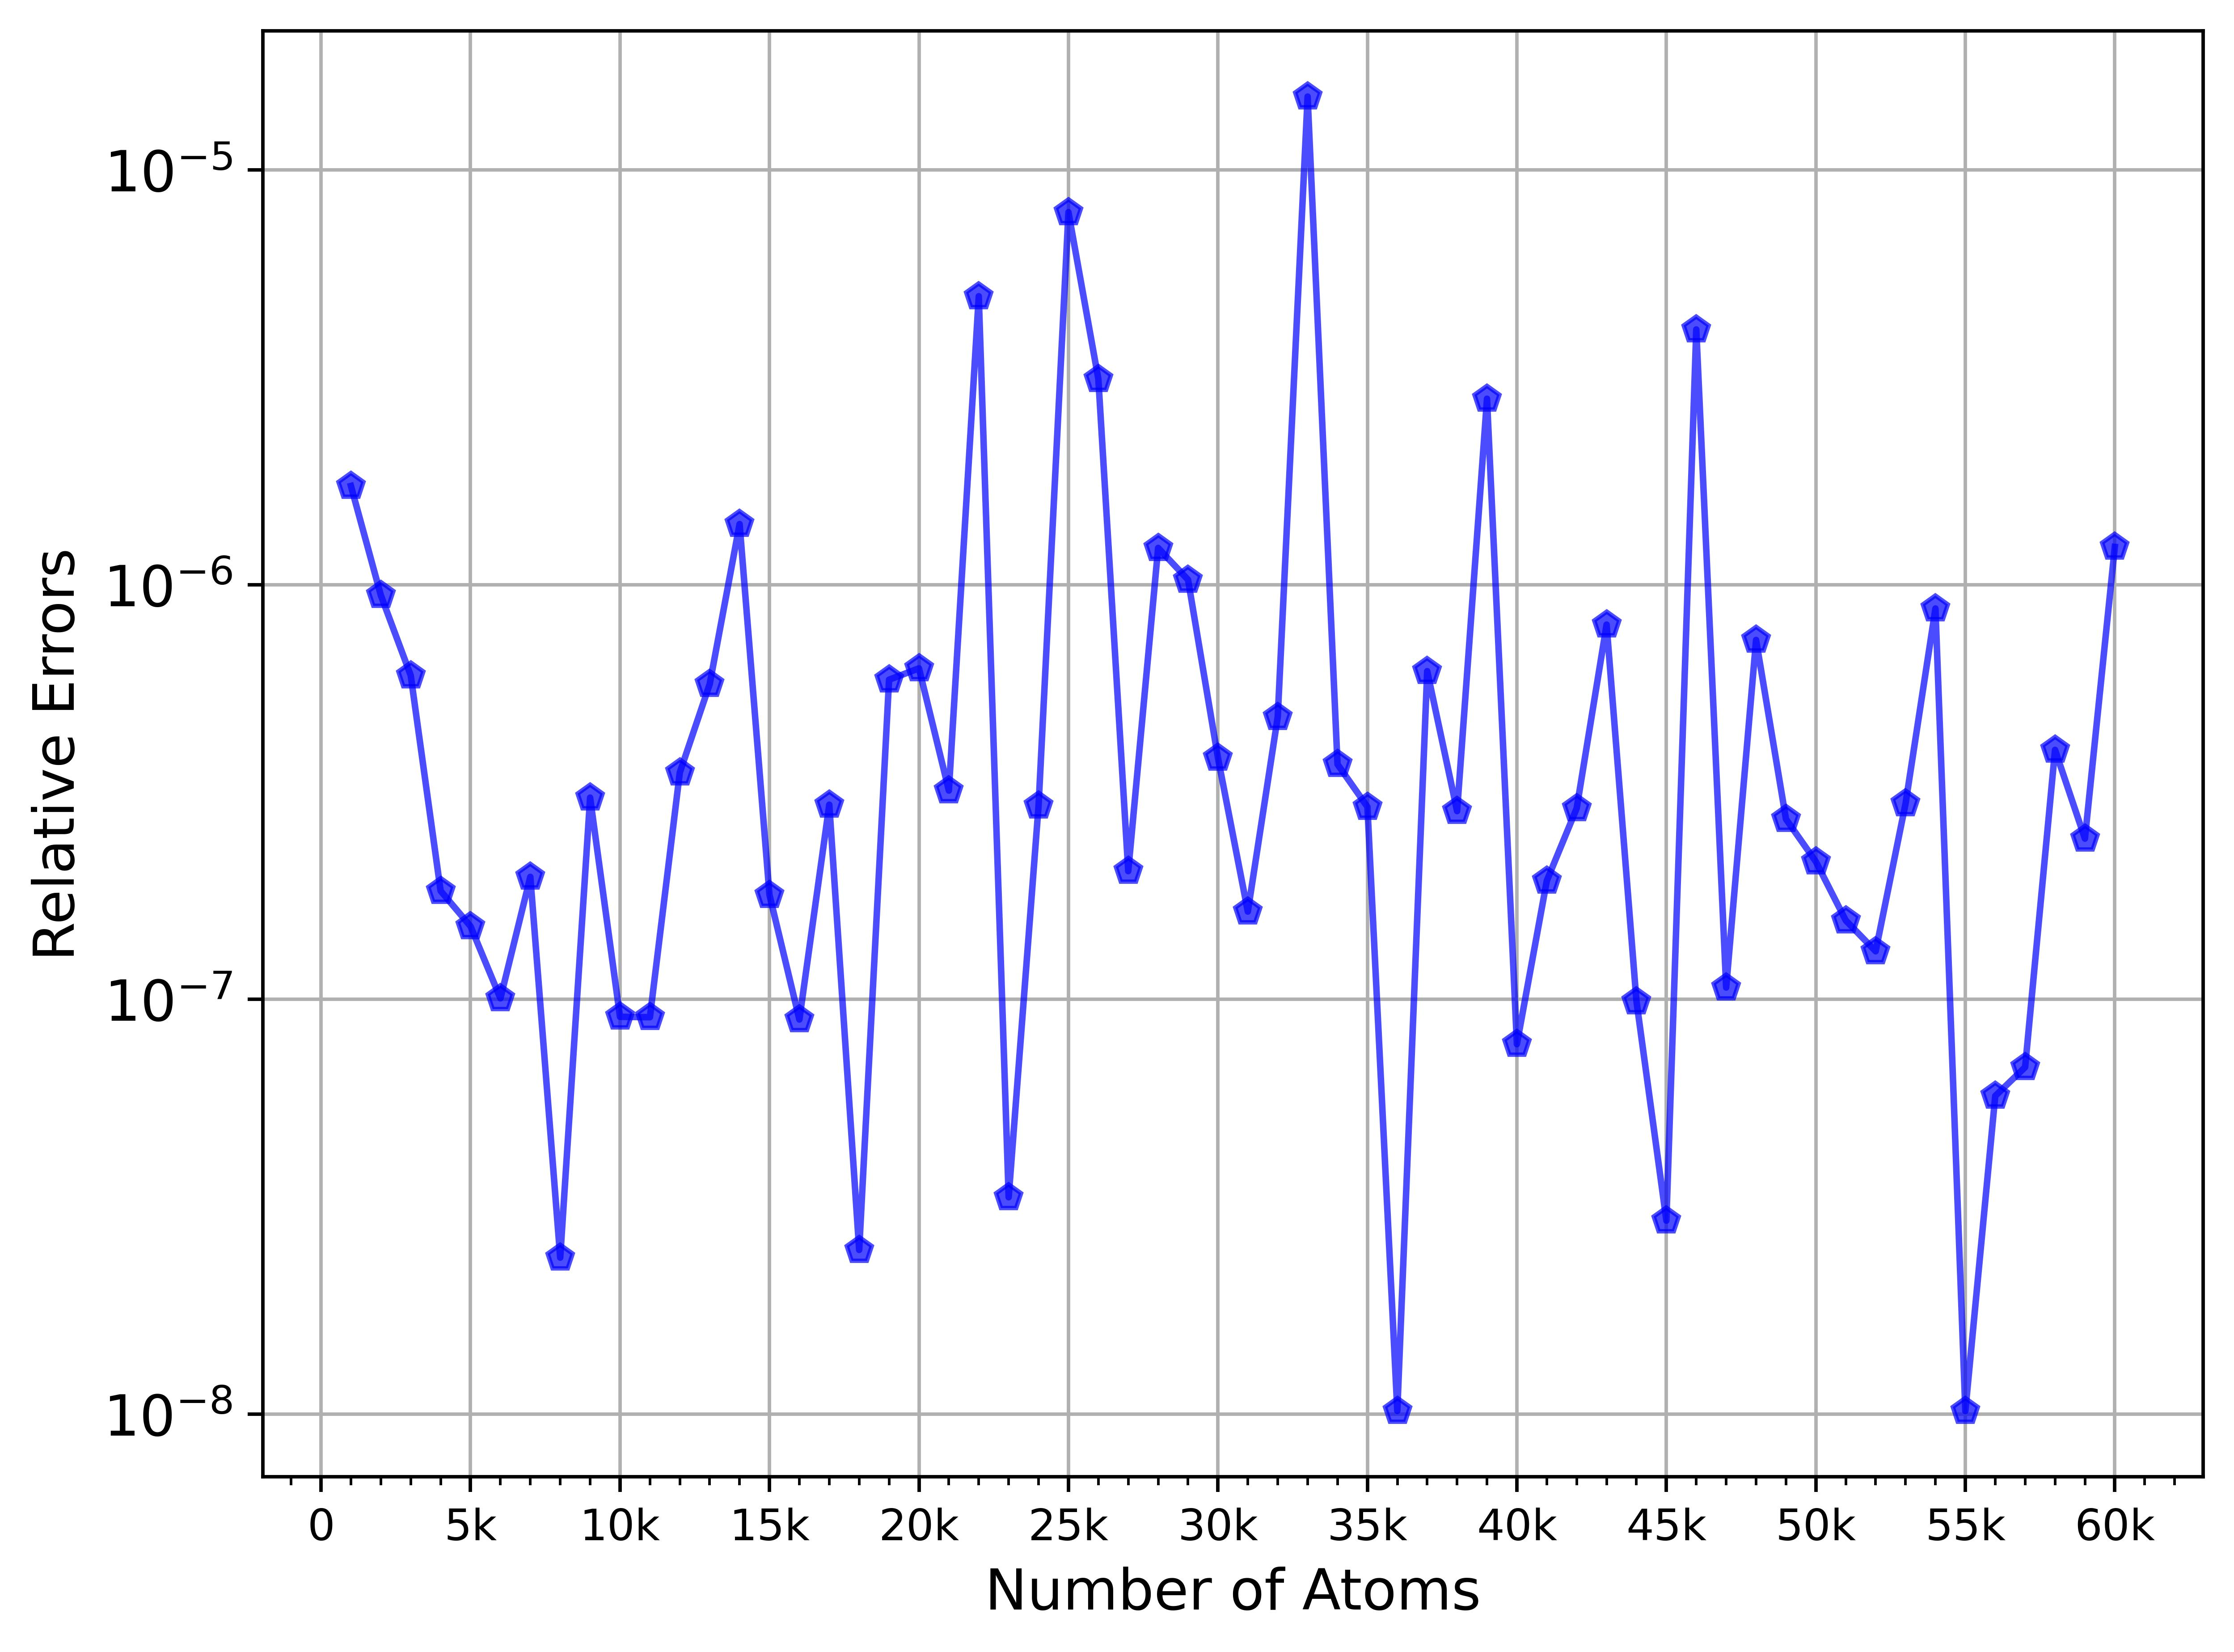
\includegraphics[width=0.75\linewidth]{images/realspaceopterrors.jpg}
    \caption{Enter Caption}
    \label{fig:enter-label}
\end{figure}
\section{Performance Scaling of the Ewald Method}
\subsection{Scaling Behaviour with System Size}
\begin{figure}[H]
    \centering
    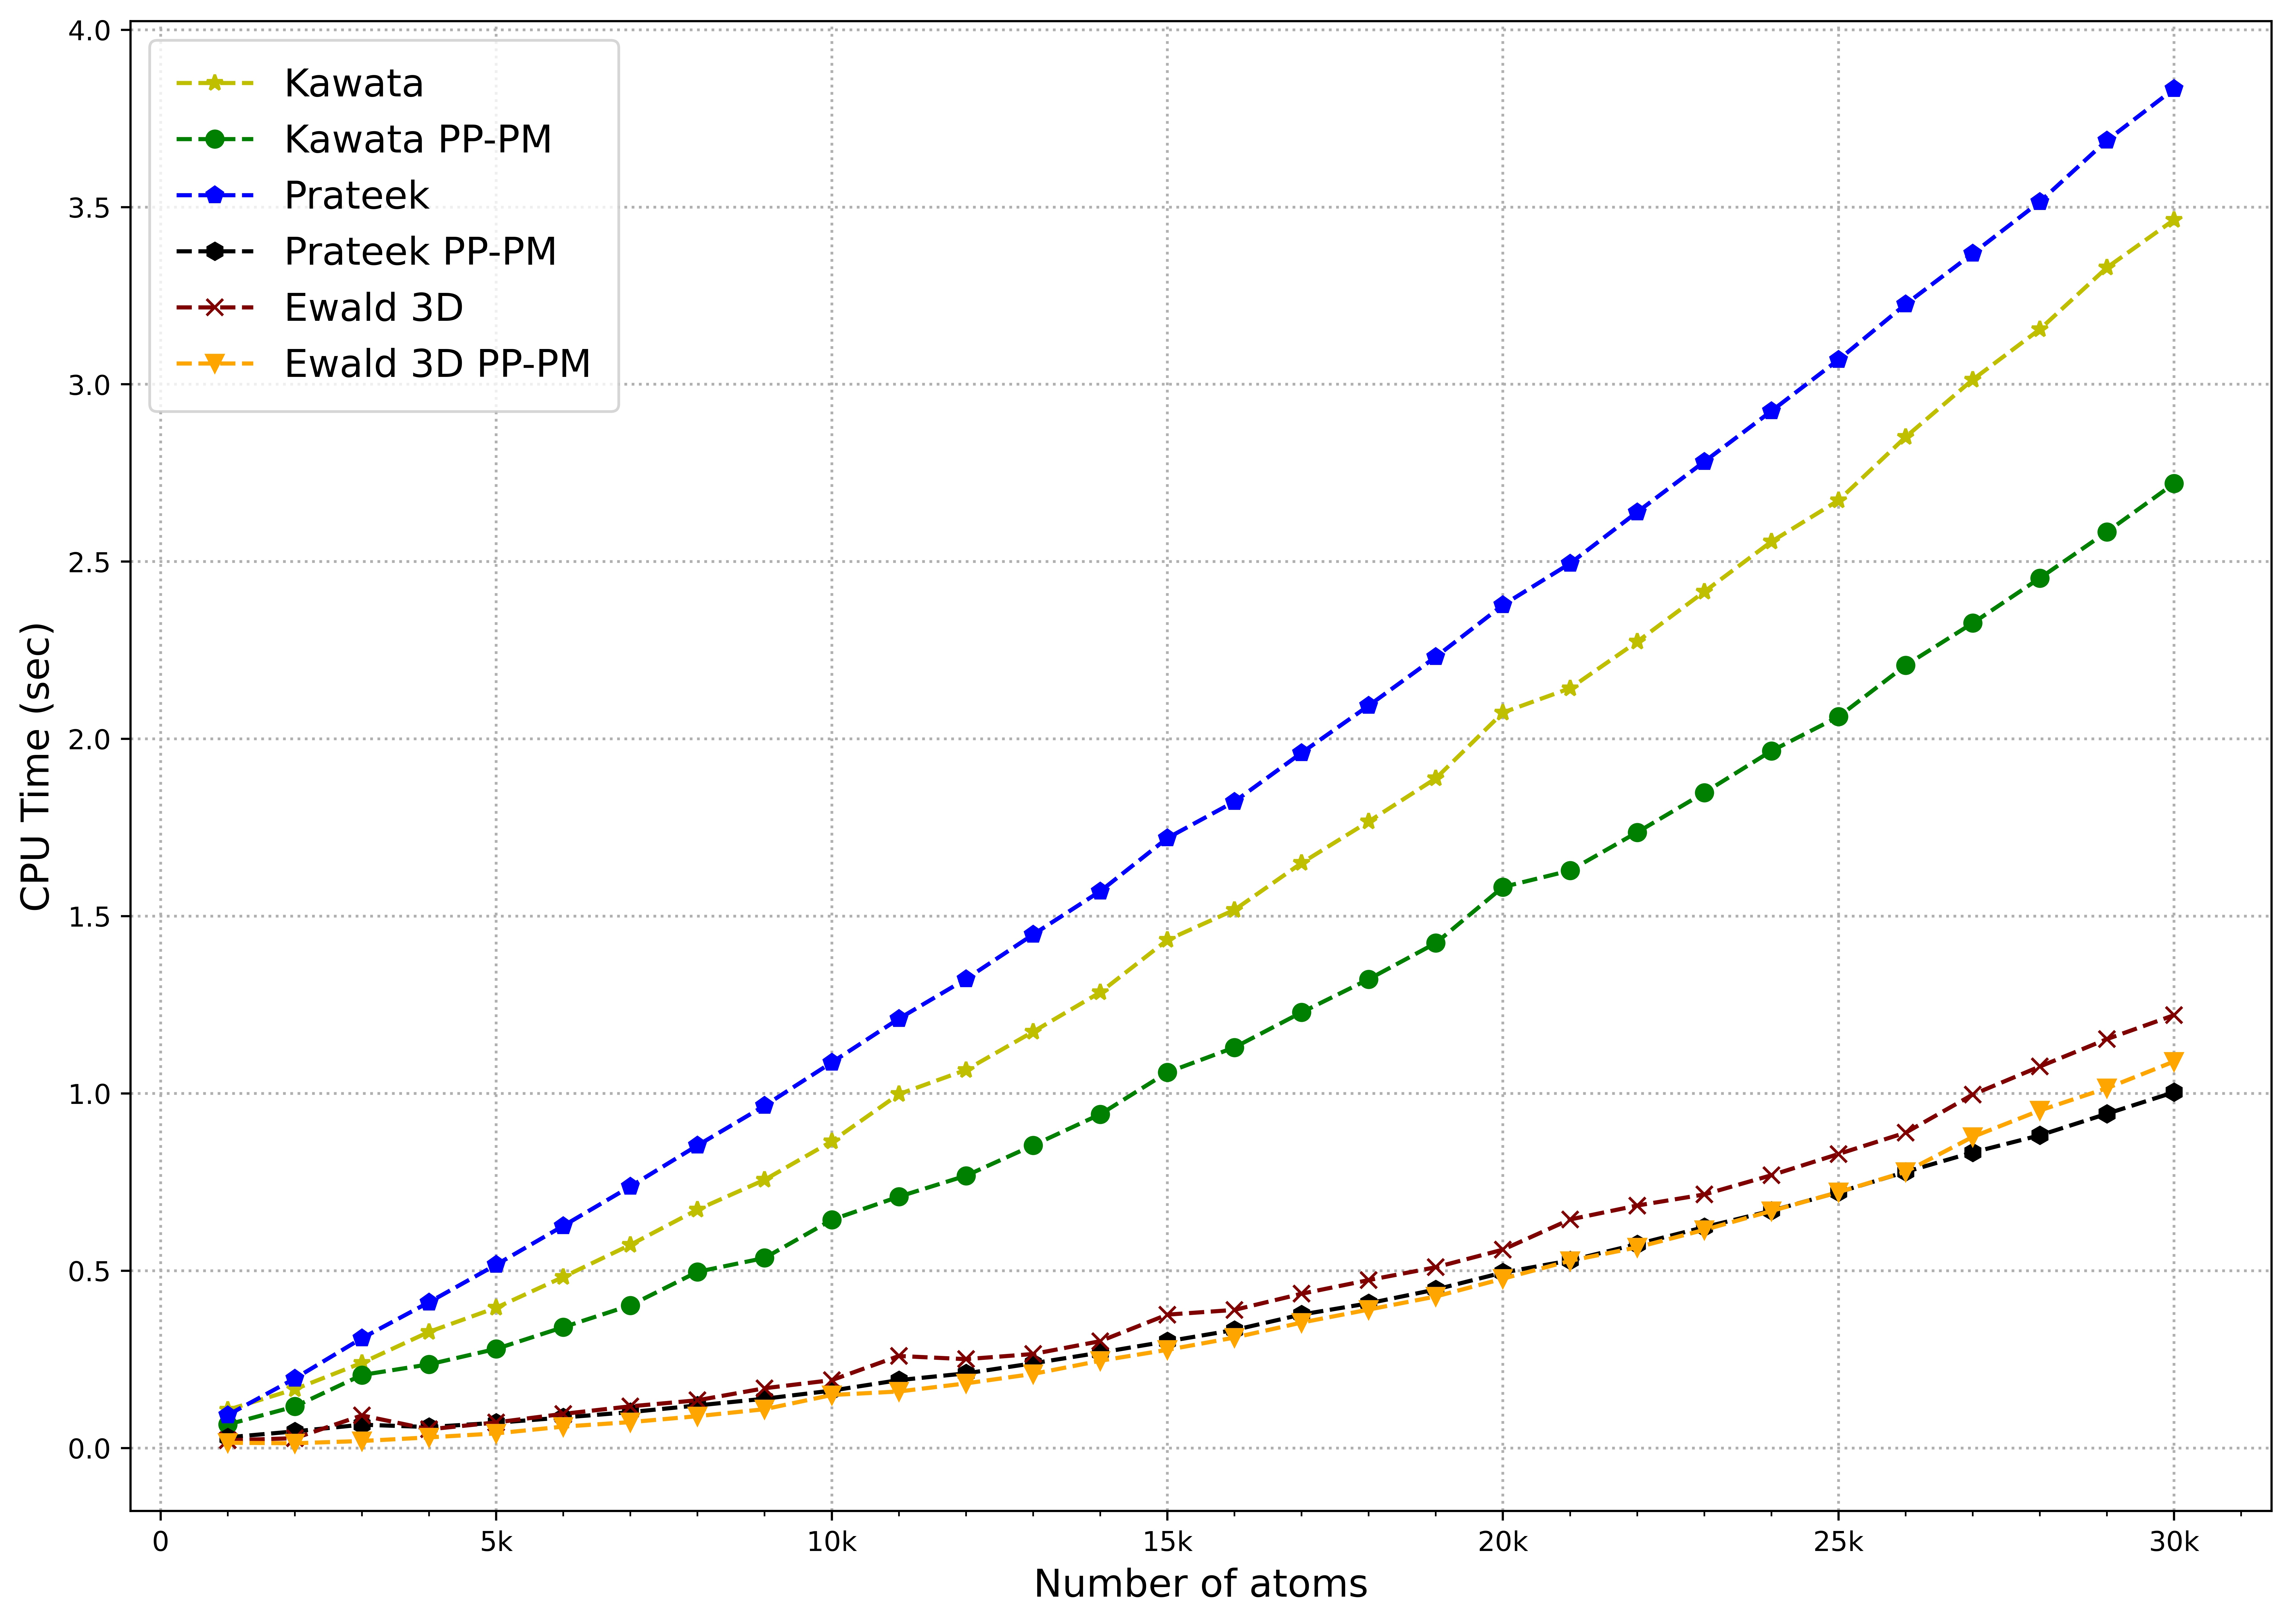
\includegraphics[width=\linewidth]{images/Result30k.jpg}
    \caption{Enter Caption}
    \label{fig:enter-label}
\end{figure}
% \subsection{Parallel Efficiency via Multi-threading}
SPME configuration
gx = 64 
gy = 64
gz = 512
nxyz = 8

% \section{Summary}